%\documentclass[pageno]{jpaper}
\documentclass{article}

\usepackage[normalem]{ulem}
\usepackage{algorithm2e}
\usepackage{amssymb}
\usepackage{amsmath}
\usepackage{float}
\usepackage{tabularx}
\usepackage{hyperref}
\usepackage{graphicx}
\usepackage{geometry}
\geometry{margin=1in}

\begin{document}

\title{Midnight Mountains - Final Project Write-up}
\author{David Paulk, Channing Huang, Christopher Giglio\\}
\date{}
\maketitle

\thispagestyle{empty}

\noindent 
$\bf{Honor \ Code}$: This paper represents our own work in accordance with University regulations.\\
Signature: /s/ David Paulk, Channing Huang, Christopher Giglio
\\ \\
\section{Introduction}
\subsection{Goal}
The aim of our project was to implement a simple video game with a focus on quality graphics.  The user's objective is to collect as many coins as possible while navigating a mountain terrain.  When the user collides with the mountain, the game ends.  As the user performs the coin-collecting task, the scene changes in several ways: a day-night cycle reflects the passage of time, the coins float about their spawn-points according to a periodic function, and the player gains speed as more coins are collected.  Also, the light emitted by the sun, the players, and the coins affects the surface of objects in the scene such as the mountainside and the fog.

\subsection{Previous Work}
Our project builds on the work of several other projects.  The Perlin noise generator used for generating heights for the mountains was adapted from \url{http://threejs.org/examples/webgl_geometry_terrain.html}.  The day-night cycle that makes the sky dynamic was implemented using [a WebGL demo] (need citation) as start code. The game music was taken from the Mario videogame (need citation).
 
\subsection{Approach}
We tried to implement normative mapping using a mountain texture.  Our implementation approach for adding this feature did not work because it could not be used simultaneously with the fog and continuously rendering the mountain texture as new mountain terrain is spawned proved to be computationally expensive, resulting in noticeable latency.

\section{Methodology}
The following subsections describe each part of the video implementation in further detail.  The parts include sky rendering, coin rendering, player perspective, navigation controls, mountain terrain spawning, collision detection, and extras (i.e. game menus and audio tracks).
\subsection{Sky Rendering}
\begin{figure}[H]
\begin{center}
\fbox{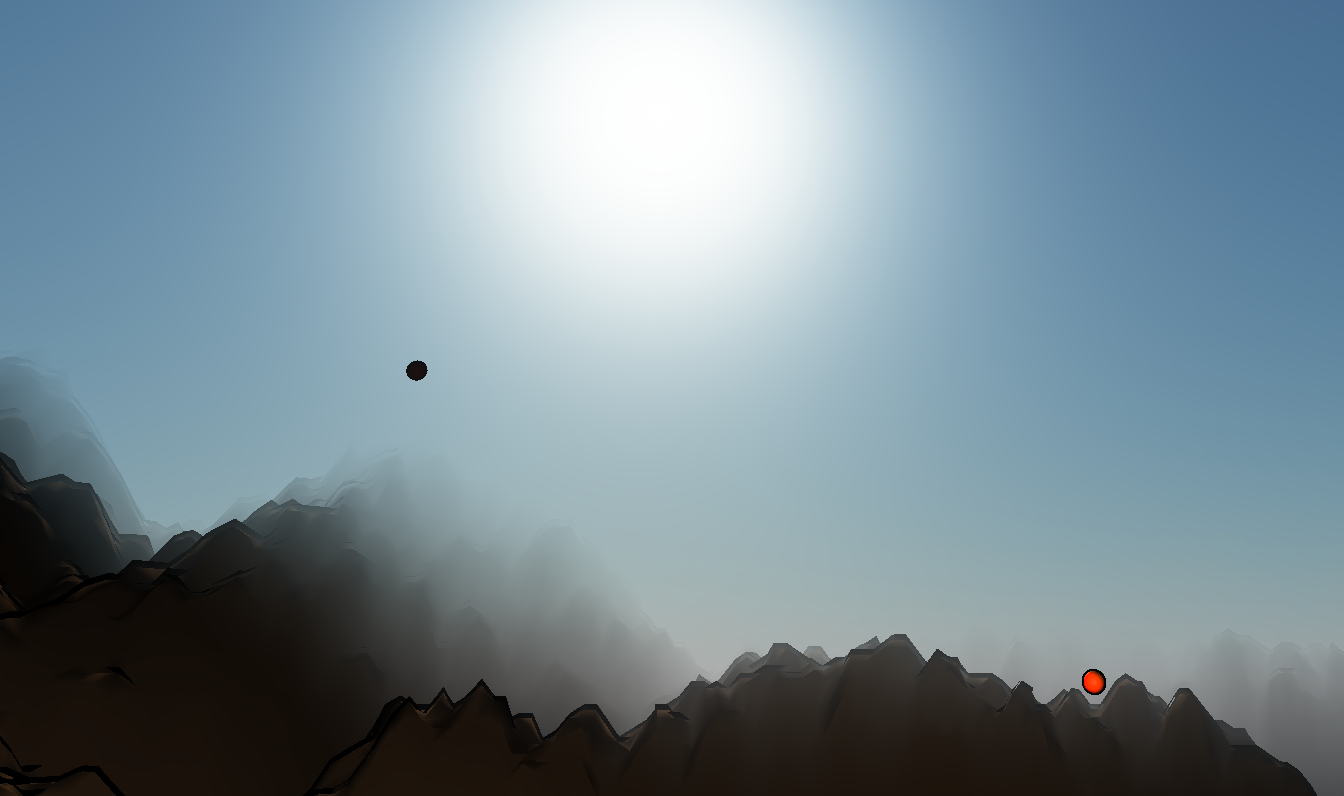
\includegraphics[width=0.47\textwidth,height=\textheight,keepaspectratio]{daytime}}
\fbox{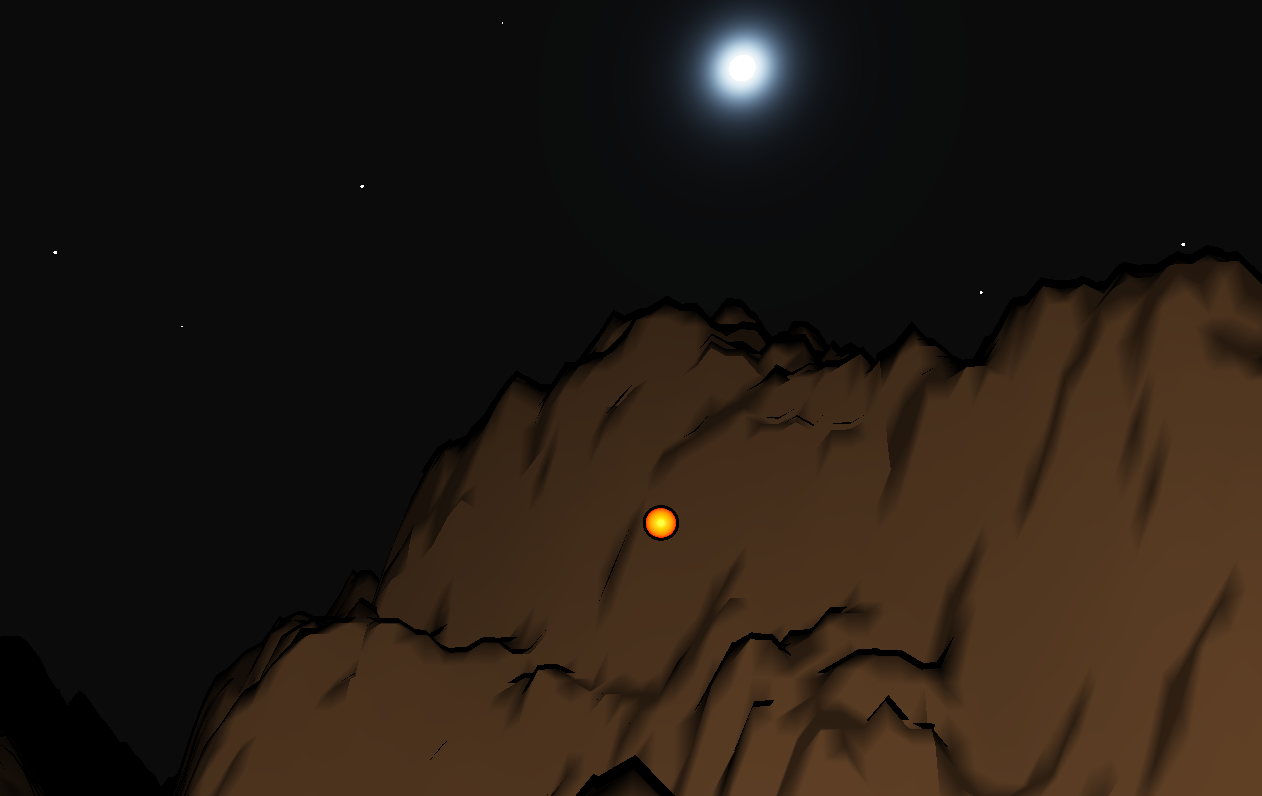
\includegraphics[width=0.44\textwidth,height=\textheight,keepaspectratio]{nighttime}}
\caption{Day-Night Cycle}
\end{center}
\end{figure}
\subsection{Coin Rendering}
It is the goal of the user to collect as many coins as possible before crashing into the mountainside.  A coin is represented in Javascript as a THREE.Object3D in the shape of a sphere and contains a THREE.PointLight to illuminate it, which is particularly convenient during the night when it is harder to navigate the terrain.  The coins are animated by moving the x, y and z coordinates of their positions according the periodic function, relative to their spawn position.
$$x += sin( time * 7 ) * 3$$
$$y += cos( time * 5 ) * 4$$
$$z += cos( time * 3 ) * 3$$
The position update is small enough so that animating them does not make it more difficult for the user to collect coins.  When the user's player collides with a coin, the score increases by one and the coin is removed from the scene.  One implementation challenge that we faced was figuring out how to spawn and update coins in a way that would avoid noticeable latency.  While one approach would be to limit the amount of memory occupied by each coin, this approach would prevent us from adding extra coin features such as lighting (glow).  A better approach for avoiding latency that we chose was to limit the number of coins present in the scene at any point in time.  We did this by first adding a maximum distance from the player that the coins can be spawned and updated at (7000 units).  Second, we limited the number of coins that could be present at any time to 10, so that after 10 coins are spawned, no more can be spawned until one or more is collected by the player.

\subsection{Player Perspective}
We tried using several player perspectives in Midnight Mountains.  First, considered a first-person perspective where the screen represents the viewpoint of the player.  Next, we implemented third-person player perspectives where the player was slightly in front of the camera and either shaped as a ring or sphere.  After implementing both types of perspective, we decided that the third-person perspective detracted from the view of the mountains and used the first-person perspective in our final product.

\subsection{Navigation Controls}
The controls are implemented with a modified THREE.FirstPersonControls. The code for looking around with the mouse is maintained; however, the movement itself is overhauled. We store the player's current velocity as a vector, and accelerate or decelerate by a constant value in each direction based on input commands. The velocity is capped, and beyond this cap, the velocity vector is scaled down to fit the cap. Additionally, the player's movement speed will decay over time if acceleration is not continued. Currently, velocity decreases by 1 percent every frame, though this is of course adjustable.

\subsection{Mountain Terrain}
The mountain terrain was initially based on the THREE.js WebGL Geometry Terrain demo at \url{http://threejs.org/examples/webgl_geometry_terrain.html}. We retain the Perlin noise generator used by the demo, but have overhauled most other aspects of the demo.

The mountain's material was made using an extended version of the MeshLambertMaterial in the THREE.js libraries. Non-photorealistic rendering of the mountains was added through toon shading and outlines. Toon shading was achieved by quantizing the $n \cdot l$ value when calculating Lambertian reflectance. Adding the outline was initially difficult, due to the many difficulties discussed in class and the need for complex ray caster operations to determine where to draw lines. However, we found a clever hack for outlining shapes that made the process significantly easier, using the method at \url{https://stemkoski.github.io/Three.js/Outline.html}. In order to add outlines, this hack duplicates all meshes, uses a basic black texture for the duplicates, and scales the duplicates up by a very small factor (we use $1.01$). Then, we add the duplicates to the scene but only render the back side of the faces. This makes it so that the only parts of the duplicate that are visible are the parts slightly beyond crests in the mesh, exactly where we want outlines.

\subsection{Mountain Terrain Spawning}
We also added infinite spawning of terrain so one can fly without worrying about hitting a boundary. In order to achieve this without using too much memory or processing power, we divide up the world into square tiles $1500$ by $1500$ units large. In the scene, we only include tiles that are within a certain distance to the player, and we dynamically add or remove tiles as necessary as the player moves. Careful offsetting within the Perlin noise function ensures that the terrain is continuous even though each tile is generated separately.

\subsection{Fog}
Fog is an important part of our game, as not only does it add ambience, but it also conceals the fact that we are adding and removing chunks of terrain as the player moves. However, adding fog proved to be a harder task than expected. Although THREE.js comes with a default implementation of fog, it only allows you to set the fog to a static color. Since we have a dynamic and multicolored background due to the day/night cycle, a static color does not suffice. Thus, we manually created ShaderMaterials for the mountain terrain and outlnes with an enhanced version of fog that calculates fog color based on position, orientation, and time in the day/night cycle.

\subsection{Collision Detection}
There are two main types of collisions we handle: collisions with the terrain and collision with coins. Collisions with the terrain are handled simply by casting a ray under the player and checking to see if there is terrain under the player. If there is not, then that means the player has intersected the mountain and we flag that the player is dead. Collisions with coins are handled by constructing an octree using the THREE.Octree library (\url{https://github.com/collinhover/threeoctree}) and inserting the coin positions into the tree. The octree can then be used to look up coins close to the player, and any coin within 200 units is considered to be picked up.

\subsection{Stars}
Stars are created by generating points at random on the surface of a sphere, and then placing white spheres at those points. The color of the star material is varied with time in order to make the transition between day and night smooth.

\subsection{Extras}
\subsubsection{Menus}
The start, pause, and death menus are implemented in HTML and overlaid atop the renderer. To pause rendering while menus are open, we stop the requestAnimationFrame loop by interrupting the animate() function and restart the loop after menus are closed.
\subsubsection{Sound}
Music and sound effects were added using the HTML5 Audio API.

\begin{figure}[H]
\begin{center}
\fbox{
\includegraphics[width=0.65\textwidth,height=\textheight,keepaspectratio]{start_screen}}
\fbox{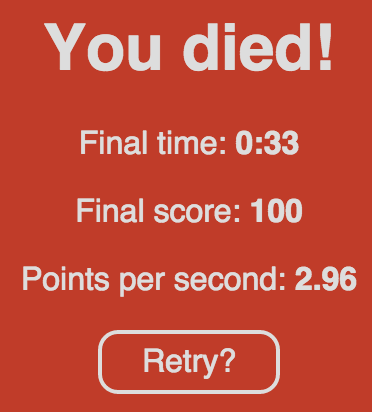
\includegraphics[width=0.3\textwidth,height=\textheight,keepaspectratio]{end_screen}}
\caption{Start Screen and End Screens}
\end{center}
\end{figure}

\section{Results}
%How did we measure success
We measured success on our project on a feature by feature basis.  As stated in Section 1.1, our core goal was to implement a simple video game with a focus on quality graphics.  When we implemented a new feature, we asked ourselves whether or not it helped us move towards our core goal, and we only added it to our final product if the answer was yes.  For example, a successful feature would enhance the landscape but not add noticable latency. Adding THREE.PointLight objects to the spheres fulfilled this criteria, but the terrain with normal mapping did not.\\

% What do our results indicate
Our final product combines the features that best supported our core goal.  Several of the features that we implemented were not added to the final product after testing the game with those features included, but the set of features that are included work well with each other to make gameplay challenging but enjoyable. For example, the terrain during the night phase can be too dark to navigate, but adding lights to the player and spheres made the night phase challenging rather than impossible.  Hence, the day-night cycle and the sphere lighting enhance the graphics of the game while also supporting each other.

%

\section{Discussion}
Overall, our game offers both fun gameplay and quality graphics. Our approach of dynamically generating terrain in fragments allows us to generate a vast landscape for the user to explore, and also offers the developer the ability to easily add further features without incurring too much computational overhead.

Additional work that could enhance the experience include adding an avatar for the character, adding additional features in the environment, and varying the scoring system. We experimented with various ways of representing the player character, but ultimately decided not to add an avatar. However, a high quality model of a bird or plane could add to the immersion. Potential additional landscape features include lakes, snow, varying textures for different mountains, vegetation, and wildlife, which could all be procedurally generated like the mountains. Particle systems could also be be used to generate weather such as rain or snow. Finally, upgrading the scoring system, perhaps with coins of varying values or rewarding players for collecting many coins in a short time span, could improve pacing of the game and excite the player.

WHAT WE LEARNED HERE

% Add what we learned

\end{document}

